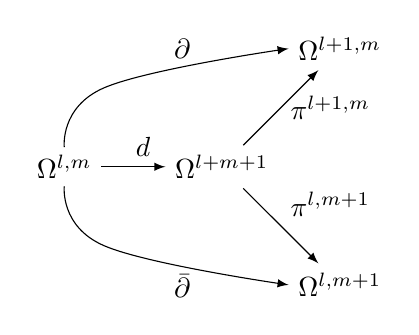
\begin{tikzpicture}

\node (v1) at (-1,0) {$\Omega^{l,m}$};
\node (v2) at (1,0) {$\Omega^{l+m+1}$};
\node (v3) at (2.5,1.5) {$\Omega^{l+1,m}$};
\node (v4) at (2.5,-1.5) {$\Omega^{l,m+1}$};

\draw [-latex] (v1) edge (v2);
\draw [-latex] (v2) edge (v3);
\draw [-latex] (v2) edge (v4);

\node [above] at (-0.,0) {$d$};

\node [right] at (1.75,0.75) {$\pi^{l+1,m}$};
\node [above right] at (1.75,-0.75) {$\pi^{l,m+1}$};

\draw [-latex] plot[smooth, tension=.7] coordinates {(-1,0.25) (-0.5,1) (1.85,1.5)};
\draw [-latex] plot[smooth, tension=.7] coordinates {(-1,-0.25) (-0.5,-1) (1.85,-1.5)};

\node [below] at (0.5,-1.25) {$\bar{\partial}$};
\node [above] at (0.5,1.25) {${\partial}$};

\end{tikzpicture}